\section{Development Process}
\subsection{Version Control}
As planned in the requirements analysis phase, Git\footnote{\url{https://git-scm.com/}} was used as the version control system.
Github\footnote{\url{https://github.com/}} was chosen as repository hosting service.

Separate repositories were created for documentation (\codeinline{doc}) and code (\codeinline{mamid}).

\subsection{Continuous Integration (Jenkins)}\label{ci}
On each push a GitHub webhook triggers a Jenkins instance\footnote{\url{https://jenkins.dogcraft.de/job/mamid/}} to build the head 
of the pushed commits. While building, Jenkins marks the commit on GitHub to indicate whether the respective target passed.

Jenkins utilizes two remote build nodes: 
\begin{itemize}
	\item A node on a Linux server
	\item A node on an OpenIndiana server 
\end{itemize}
Therefore artifacts for both Linux and OpenIndiana can be produced and tested.

Jenkins executes the following Makefile targets on both nodes:
\begin{itemize}
	\item \codeinline{check\_format}
	\item \codeinline{vet}
	\item \codeinline{test}
	\item \codeinline{build}
	\item \codeinline{cover}
\end{itemize}
\subsection{Workflow}
Each change of the code have to be implemented in a separate feature branch since the master branch is protected on GitHub. The protection 
only allows changes to be pushed on master if the following constraints are fulfilled:
\begin{itemize}
	\item The change can be applied fast forward
	\item The change passes all required checks on the \hyperref[ci]{CI}, which are:
	\begin{itemize}
		\item the \codeinline{check\_format} makefile target succeeds
		\item the \codeinline{vet} makefile target succeeds
		\item the \codeinline{test} makefile target succeeds on both Linux and OpenIndiana
		\item the \codeinline{build} makefile target succeeds
	\end{itemize}
\end{itemize}

\subsection{Local Staging Environment}
A local staging environment can be spawned using Docker and the makefile target \codeinline{testbed\_up}.

The target
\begin{itemize}
  \item creates a host-only test network
  \item builds \mamid in a container
  \item builds Docker images with the newly built binaries for master, slave and notifier
  \item starts Docker containers: 1 master, 1 PostgreSQL instance, 3 slaves, 1 notifier
\end{itemize}

Re-executing the \codeinline{testbed\_up} wipes the previously created environment, allowing for quick reproducible testing of changes.

\subsection{Communication}

Team communication was handled mostly via the Slack\footnote{\url{https://slack.com}} chat platform.
Automatic posting of commits and CI results into separate channels was configured to increase overview of the team's activity.

GitHub's issue tracker was used to track bugs, enhancements and deviations from the design document.
However, bugs that were fixed as they were encountered were not necessarily tracked in order to reduce time overhead.

\subsection{Distribution of Work}

The first step of the implementation phase was analyzing the API dependencies between \mamid components:

\begin{figure}[h]
\centering
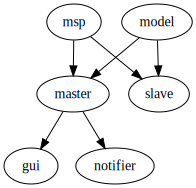
\includegraphics[height=5cm]{assets/module_graph}
\caption{Module Dependency Graph}
\end{figure}

\begin{itemize}
  \item Since the Master API was fully specified in the design document, GUI and notifier could be implemented indepenently.

  \item MSP and Model are mostly static datastructures and a simple transport mechanism.
        It was assumed they could be implemented quickly.

  \item Master and slave do not depend on each other code-wise, hence implementation could be parallelized, too.
\end{itemize}

Given these assumptions, it was attempted to distribute the work fairly between the team members, assuming cleanly separated
responsibilities would increase speed \& motivation through independent \& parallel work.

\begin{figure}[h]
\centering
\begin{tabular}{l|l}
        Component & Name\\
        \hline
        msp       & Anton\\
        model     & Christian\\
        master    & Anton, Christian\\
        slave     & Bob\\
        gui       & Janis\\
        notifier  & Niklas, Janis\\
\end{tabular}
\caption{Original Distribution of Work}
\end{figure}

This plan played out as follows:

\begin{itemize}
\item Initial versions of MSP and Model were implemented in a few days.
\item The master with its \textit{repository pattern} (independent modules with central database) proved as difficult to implement, as
      explained in \ref{di}.
\item The GUI implementation was straight forward. In particular, the AngularJS framework turned out to be a pleasant choice.
\item The notifier implementation was equally straight forward.
\item The initial slave implementation was finished early.
\end{itemize}

Two weeks prior to the phase deadline, integration of the individual components began:

\begin{itemize}
\item GUI and notifier worked flawlessly with the master API. The fact that the originally defined API endpoints were not changed
                but only new ones added was beneficial (see \ref{di:opneeds}).
\item Model and MSP worked well, apart from the consequences of migrating to PostgreSQL late in the implementation phase
        (see \ref{di:dbchanges}).
\item Integration of master and slave revealed flaws in the assumptions made about MongoDB in the design phase:
        \begin{itemize}
                \item a lot of unexpected Mongod behavior as described in \ref{di:replsetconfig} was only discovered at the
                        time of integration and required time-consuming test setups and debugging sessions.
                \item the addition of the keyfile requirement consumed a significant amount of time (3 days) in the
                       last seven days of the implementation phase (see \ref{di:keyfiles})
        \end{itemize}
\end{itemize}

The main conclusion drawn from this integration subphase is that master and slave should have been tested together earlier, allowing for
discovery and possibly more elegant handling of unexpected MongoDB behavior, as described in section \ref{di}.
